\documentclass[a4paper,12pt]{article} % тип документа

% Поля страниц
\usepackage[left=2.5cm,right=2.5cm,
    top=2cm,bottom=2cm,bindingoffset=0cm]{geometry}
    
%Пакет дял таблиц   
\usepackage{multirow} 
    
%Отступ после заголовка    
\usepackage{indentfirst}


% Рисунки
\usepackage{floatrow,graphicx,calc}
\usepackage{wrapfig}

%%% Работа с картинками
\usepackage{graphicx}  % Для вставки рисунков
\graphicspath{{images/}{images2/}}  % папки с картинками
\setlength\fboxsep{3pt} % Отступ рамки \fbox{} от рисунка
\setlength\fboxrule{1pt} % Толщина линий рамки \fbox{}
\usepackage{wrapfig} % Обтекание рисунков и таблиц текстом

% Создаёем новый разделитель
\DeclareFloatSeparators{mysep}{\hspace{1cm}}

% Ссылки?
\usepackage{hyperref}
\usepackage[rgb]{xcolor}
\hypersetup{				% Гиперссылки
    colorlinks=true,       	% false: ссылки в рамках
	urlcolor=blue          % на URL
}


%  Русский язык
\usepackage[T2A]{fontenc}			% кодировка
\usepackage[utf8]{inputenc}			% кодировка исходного текста
\usepackage[english,russian]{babel}	% локализация и переносы




% Математика
\usepackage{amsmath,amsfonts,amssymb,amsthm,mathtools}

%%% Дополнительная работа с математикой
\usepackage{amsmath,amsfonts,amssymb,amsthm,mathtools} % AMS
\usepackage{icomma} % "Умная" запятая: $0,2$ --- число, $0, 2$ --- перечисление


% Что-то 
\usepackage{wasysym}


\begin{document}
\begin{center}
	\footnotesize{МОСКОВСКИЙ ФИЗИКО-ТЕХНИЧЕСКИЙ ИНСТИТУТ\\(НАЦИОНАЛЬНЫЙ 			ИССЛЕДОВАТЕЛЬСКИЙ УНИВЕРСИТЕТ)}\\
	\footnotesize{ФИЗТЕХ-ШКОЛА РАДИОТЕХНИКИ И КОМПЬЮТЕРНЫХ ТЕХНОЛОГИЙ\\}
	\hfill \break
	\hfill \break
	\hfill \break
	\hfill \break
	\hfill \break
	\hfill \break
\end{center}

\begin{center}   
    \hfill \break
	\hfill \break
	\hfill \break
	\hfill \break
	\hfill \break
	\hfill \break
	\hfill \break
	\hfill \break
	\hfill \break
	\hfill \break
	\hfill \break
	\large{Лабораторная работа № 4.4.1\\\large{\textbf{Амплитудная дифракционная решетка}}}\\
	\hfill \break
	\hfill \break
	\hfill \break
	\hfill \break
	\hfill \break
	\hfill \break
	\hfill \break
	\hfill \break
	\hfill \break
	\hfill \break
	\hfill \break
	\begin{flushright}
		Климова Екатерина\\
		Группа Б01-108
	\end{flushright}
	\hfill \break
\end{center}
\hfill \break
\hfill \break
\begin{center}
	Долгопрудный, 2023 г.
\end{center}
\thispagestyle{empty}

\newpage
\hfill \break
\textbf{Цель работы:} знакомство с работой и настройкой гониометра, определение спектральных характеристик амплитудной решетки.
\hfill \break
\hfill \break
\textbf{В работе используются:} гониометр; ртутная лампа; амплитудная решетка; призменный уголковый отражатель; щель с микрометрическим винтом.

\section{Аннотация}
\hfill \break В работе предлагается отъюстировать гониометр, исследовать спектр ртутной лампы в $\pm 1$ порядках и дисперсию решетки в разных порядках, оценить влияние ширины пучка на разрешающую способность.

\section{Теоретические сведения}
\subsection{Амплитудная дифракционная решетка}
\hfill \break Амплитудную решетку можно представить в виде непрозрачного экрана, в котором прорезано большое число $N$ параллельных щелей $-$ штрихов (рис. 1). Постоянство расстояний между штрихами $d$ (период решетки, или шаг решетки) и шириной штриха $b$ должно выдерживаться с большой точностью.

\begin{wrapfigure}{r}{0.2\textwidth}
\begin{center}
    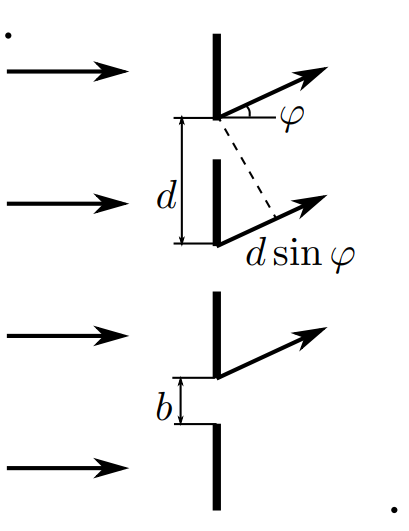
\includegraphics[width=1\textwidth]{4.4.1_1.png}
    \textbf{Рис. 1.} Дифракция световой волны на амплитудной решетке
\end{center}
\end{wrapfigure}

\hfill \break Наблюдение изображения спектра проводится с помощью зрительной трубы, настроенной на бесконечность. В этом случае амплитуда и интенсивность поля световой волны определяются углом $\varphi$ между нормалью к решетке и направлением дифрагировавших лучей. Будем считать, что амплитуды всех интерферирующих волн одинаковы, то есть фиксирована амплитуда падающей волны и постоянна площадь всех штрихов. Интенсивность дифрагированного света максимальна для углов $\varphi_{m}$, при которых волны, приходящие в точку наблюдения от всех щелей, оказываются в фазе:

\begin{equation}\label{ linkname }
d\sin{\varphi}_{m} = m\lambda.
\end{equation}

\hfill \break Величина $m = 0, \pm 1, \pm 2, \pm 3, ...$ называется \textit{порядком спектра}.

\hfill \break Рассмотрим качественный пример. Пусть падающее на решетку излучение содержит две спектральные линии одинаковой интенсивности. Одну линию условно назовем <<красной>>, а другую <<фиолетовой>>. Длина волны <<красной>> линии больше, чем длина волны <<фиолетовой>>. Изображение спектра приведено на рис. 2. Для угла дифракции $\varphi_{0} = 0 \text{ } (m = 0)$, когда ось зрительной трубы параллельна оси коллиматора, наблюдается наложение изображений входной щели коллиматора в <<красном>> и <<фиолетовом>> цвете друг на друга. При повороте зрительной трубы вокруг решетки в поле зрения возникает <<фиолетовая>> щель коллиматора, затем <<красная>> и т.д. Для малых углов дифракции $\varphi_{m}$ угловое расстояние между порядками $\varphi_{m+1} - \varphi_{m} \approx \lambda/d$ пропорционально длине волны, поэтому <<фиолетовые>> линии следуют чуть чаще, чем <<красные>>, и возможна ситуация, когда они вновь налагаются друг на друга (на рис. 2 это происходит при  $m = 5$ для <<красной>> линии и $m = 6$ для <<фиолетовой>>).

\begin{center}
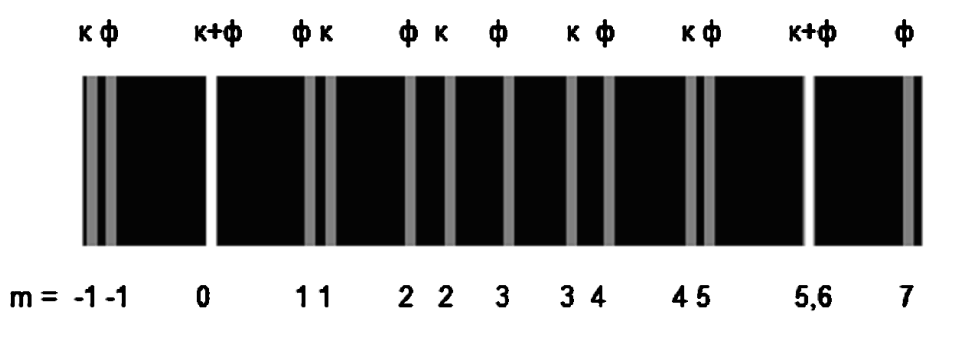
\includegraphics[width=0.65\textwidth]{4.4.1_2.png}\\
\textbf{Рис. 2.}  Изображение спектра двух линий\\ 
\end{center}

\hfill \break Уточним форму распределения интенсивности света наблюдаемой спектральной линии. Для очень узкой входной щели коллиматора эта форма зависит от числа штрихов решетки $N$, шага решетки $d$ и ширины ее штриха $b$. Пусть интенсивность квазимонохроматического света (длина волны $\lambda$) равна $I_{0}$ [Вт/$\text{см}^2$]. Учет дифракции Фраунгофера на отдельной щели решетки и когерентного сложения полей от всех штрихов решетки дает следующее выражение для мощности света на единицу высоты изображения спектральной линии в малом интервале углов дифракции $d\varphi$:

$$
dW = I_{0} \frac{b^2}{\lambda} \left( \frac{\sin{\left(\frac{\pi}{\lambda}\sin{\varphi} \right)}}{\frac{\pi}{\lambda} b\sin{\varphi}}\right)^2 \cdot \left( \frac{ \sin{ \left( \frac{\pi}{\lambda} Nd\sin{\varphi} \right) } } { \sin{ \left( \frac{\pi}{\lambda} d \sin{\varphi} \right) } } \right)^2 d\varphi.
$$

\hfill \break Здесь величина $W$ имеет размерность [Вт/см].

\hfill \break В этом выражении множитель

$$
\left( \frac{\sin{\left(\frac{\pi}{\lambda}\sin{\varphi} \right)}}{\frac{\pi}{\lambda} b\sin{\varphi}}\right)^2
$$

\hfill \break описывает дифракцию света на отдельной щели решетки (рис. 3а). Для ширины щели $b \gg \lambda$ область углов центрального, или главного максимума огреничена отрезками $|\varphi| \leq \lambda/b$ (координаты нулей распределения). В этой области сосредоточено около $90 \%$ мощности света. Множитель

$$
\left( \frac{ \sin{ \left( \frac{\pi}{\lambda} Nd\sin{\varphi} \right) } } { \sin{ \left( \frac{\pi}{\lambda} d \sin{\varphi} \right) } } \right)^2
$$

\hfill \break описывает когерентное сложение полей от $N$ штрихов (рис. 3б). Максимумы этого распределения возникают при обращении знаменателя в ноль, что имеет место при выполнении условия (1). Область локализации мощности отдельного максимума $|\delta \varphi | \leq \lambda/Nd$ много меньше ширины главного дифракционного максимума $2\lambda / b$. На рис. 3в приведена форма спектра квазимонохроматического света.

\hfill \break Мощность света на единицу высоты изображения спектральной линии в порядке $m$:

$$
W_{m} \approx I_{0} \frac{b^2}{\lambda} N \left( \frac{ \sin{ \pi \frac{b}{d} m } } { \pi \frac{b}{d} m } \right)^2.
$$

\hfill \break Суммарная мощность всех порядков $\approx I_{0}Nb$ и равна мощности света за решеткой. Разумное ограничение на рабочий порядок спектра $m_{p}$: $0 < |m_{p}| < d/b$, то есть порядок не нулевой и лежит в области главного дифракционного максимума отдельной щели.

\hfill \break Отметим, что наблюдение в опытах идеальных линий, приведенных на рис. 3в, весьма затруднительно, так как угловой размер щели коллиматора $l/f$ ($l$ $-$ ширина щели, $f$ $-$ фокусное расстояние колиматора) должен быть заметно меньше ширины линии $\lambda/Nd$. Как уменьшение ширины щели $l$, так и уменьшение размера решетки $Nd$ приводят к большим потерям света. Практически при измерениях наблюдается слегка размытое изображение щели коллиматора.

\begin{center}
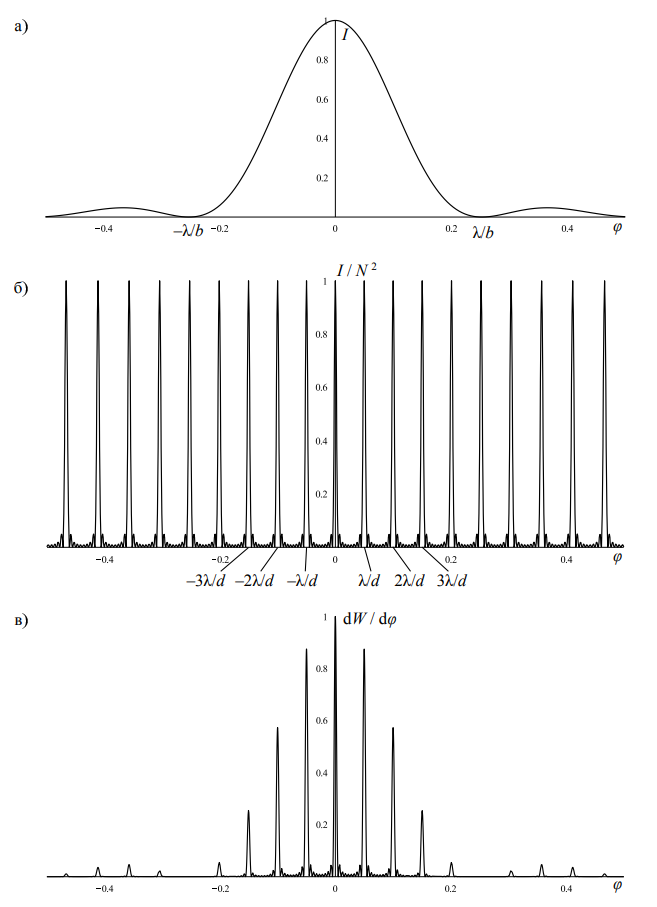
\includegraphics[width=0.65\textwidth]{4.4.1_21.png}\\
\textbf{Рис. 3.}  Дифракция света на решетке ($\lambda / b \approx 0.25, \lambda / d \approx 0.05$). Зависимость интенсивности света от угла: а) дифракция на отдельной щели; б) дифракиця на решетке в пределе бесконечно узких щелей; в) распределение мощности света на единицу высоты изображения, отнесенное к малому диапазону углов\\ 
\end{center}

\subsection{Угловая дисперсия}
\hfill \break \textbf{Угловая дисперсия} $D(\lambda)$ характеризует угловое расстояние между близкими спектральными линиями:

\begin{equation}\label{ linkname }
D(\lambda) = \frac{d\varphi}{d\lambda}.
\end{equation}

\hfill \break Угловая дисперсия позволяет определить минимальное расстояние между ячейками приемного устройства: если требуется разрешить две спектральные линии с разностью длин волн $\delta \lambda$, то расстояние между элементами приемного устройства должно быть заметно меньше $D \delta \lambda f$, где $f$ $-$ фокусное расстояние объектива зрительной трубы. 

\hfill \break Выражение для угловой дисперсии дифракционной решетки:

\begin{equation}\label{ linkname }
D = \frac{d \varphi}{d \lambda} = \frac{m}{d \cos{\varphi}} = \frac{m}{\sqrt{d^2 - m^2\lambda^2}}.
\end{equation}

\hfill \break Дисперсия возрастает с увеличением порядка спектра. Для малых углов дифракции $\varphi \ll 1$  дисперсия пропорциональна порядку спектра: $D \approx m/d$.

\subsection{Разрешающая способность}

\begin{wrapfigure}{l}{0.35\textwidth}
\begin{center}
    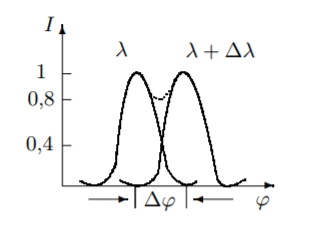
\includegraphics[width=1\textwidth]{4.4.1_3.png}
    \textbf{Рис. 4.} К определению разрешающей способности дифракционной решетки 
\end{center}
\end{wrapfigure} 

\hfill \break Рассмотрим изображения спектра для двух узких спектральных линий с длинами волн $\lambda$ и $\lambda + \delta \lambda$. Для минимального значения $\delta \lambda$, которое может быть определено по результатам измерений, вводят важнейшую характеристику спектрального прибора $-$ \textbf{разрешающую способность}:

\begin{equation}\label{ linkname }
R = \frac{\lambda}{\delta \lambda}.
\end{equation}

\hfill \break Рассмотрим физические ограничения разрешающей способности. Начнем уменьшать размер щели. В начале этого процесса будет уменьшаться интенсивность линий и их ширина. Начиная с некоторого момента будет уменьшаться только интенсивность, а ширина линий изменяться не будет. Достигнут физический предел ширины линии, и он определяется дифракцией света на апертуре решетки. Определим угловое расстояние между максимумом линии и ее первым нулем $-$ полуширину линии $\dela \varphi$. Пусть на решетку, состоящую из $N$ штрихов, падает параллельный пучок света перпендикулярно ее поверхности. Если $N = 2$, то две волны погасят друг друга, если между ними возникнет разность хода $\lambda/2$, если $N = 3$, то $\lambda/3$. В общем случае $N$ штрихов для полуширины линии $\delta \varphi$ получаем уравнение, решение которого совместно с (1) при $\delta \varphi \ll 1$ имеет вид

$$
d\sin{(\varphi_{m} + \delta \varphi)} = m\lambda + \frac{\lambda}{N},
$$

$$
\delta \varphi = \frac{\lambda}{Nd\cos{\varphi}_{m}},
$$

\hfill \break здесь $Nd\cos{\varphi}_{m}$ $-$ видимый под углом $\varphi_{m}$ размер решетки. Угловое расстояние между двумя линиями определяется дисперсией:

$$
\Delta \varphi \approx D \delta \lambda = \frac{m}{d\cos{\varphi}_{m}} \delta \lambda.
$$

\hfill \break Для сравнения между собой различных спектральных приборов Релей предложил приравнять полуширину $\delta \varphi$ и расстояние между линиями $\Delta \varphi$. Критерий Релея удобен для различных оценок. Согласно ему для дифракционных решеток разрешающая способность определяется порядком спектра и числом штрихов:

\begin{equation}\label{ linkname }
R = Nm.
\end{equation}
 
\hfill \break Здесь под $N$ следует понимать число одновременно работающих штрихов решетки, которое, вообще говоря, не равно суммарному числу штрихов освещенного участка решетки. Число штрихов $N$ определяется качеством реплики, размером источника света и т.д. 

\hfill \break На рис. 4 показана зависимость от угла интенсивности двух линий. Форма линий определяется дифракцией Фраунгофера на апертуре решетки, угловая координата максимума одной линии совпадает с первым минимумом для другой (условие Релея). Основная числовая характеристика условия Релея $-$ отношение интенсивности света в провале между линиями к максимальному значению. Численное значение этой характеристики для решетки равно $2 \left( \frac{\sin{\pi/2}}{\pi/2} \right) \approx 0.81$.

\subsection{Дисперсионная область}
\hfill \break При большой ширине спектра спектры различных порядков могут накладываться друг на друга. Предельная ширина спектрального интервала $\Delta \lambda$, при которой спектры соседних порядков перекрываются своими границами, называется \textbf{дисперсионной областью}. При этом $m(\lambda + \Delta \lambda) = (m + 1)\lambda$ и дисперсионная область

\begin{equation}\label{ linkname }
\Delta \lambda = \frac{\lambda}{m}.
\end{equation}

\hfill \break Ограничений на оптические спектры не возникает при использовании дифракционных решеток, работающих в первом порядке спектра, для них $\Delta \lambda \approx \lambda$.

\section{Экспериментальная установка}

\begin{center}
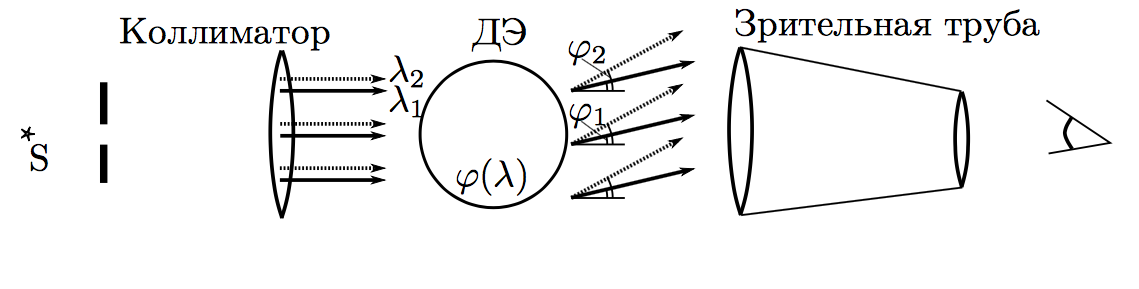
\includegraphics[width=0.75\textwidth]{4.4.1_4.png}\\
\textbf{Рис. 5.}  Условная схема экспериментальной установки: источник-коллиматор $-$ диспергирующий элемент $-$ зрительная труба\\ 
\end{center}

\hfill \break Условная схема экспериментальной установки представлена на рис. 5. В ходе работы будет производиться исследование спектра ртутной лампы. Схема гониометра, за которым находится лампа, представлена на рис. 6:

\begin{center}
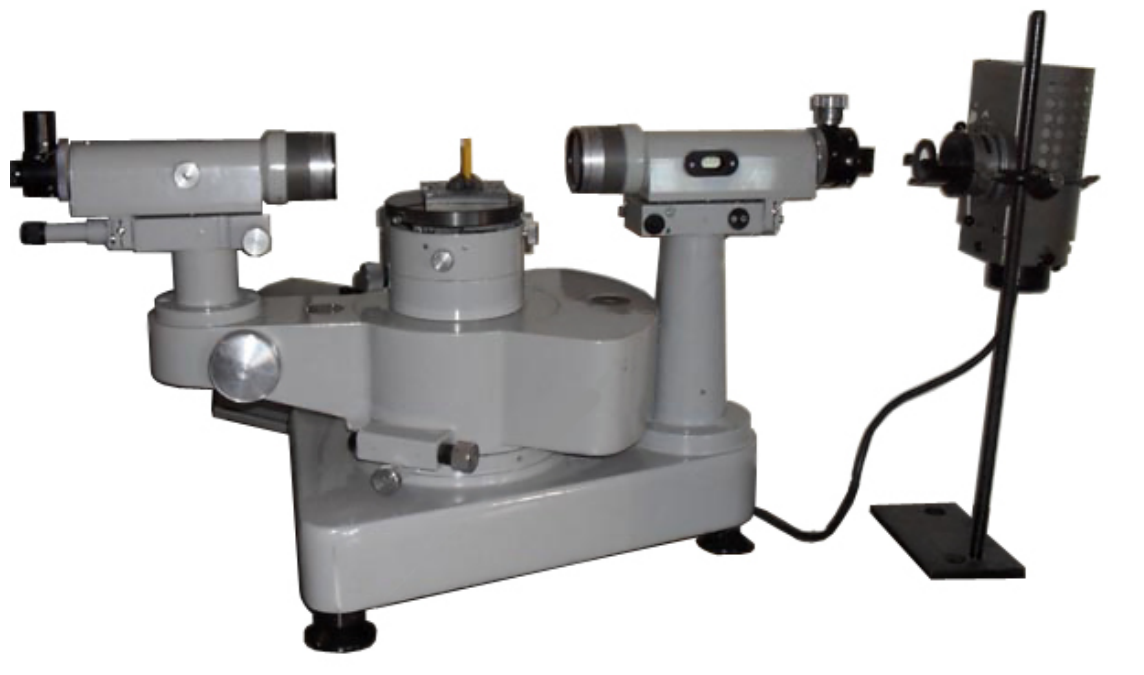
\includegraphics[width=0.75\textwidth]{4.4.1_5.png}\\
\textbf{Рис. 6.}  Устройство гониометра\\ 
\end{center}

\section{Ход работы}
\hfill \break Подготовим приборы к работе: проведем юстировку гониометра, установим начало отсчета, руководствуясь правилами ТО, настроим зрительную трубу и установим решетку. Подберем ширину входной щели так, чтобы ширина желтой спектральной линии была чуть больше промежутка между линиями двойного штриха окуляра зрительной трубы. Установим высоту щели, удобную для измерений (при короткой щели плохо виден двойной штрих, при слишком высокой $-$ мешает кривизна изображения). 

\hfill \break Измерим угловые координаты спектральных линий ртути в $\pm 1$ порядках и занесем результаты в таблицу 1:

\begin{center}
\begin{tabular}{|c|c|c|c|c|c|c|}\hline
Порядок & Цвет & $ \lambda $, нм & $ \varphi $ & $ \sin{\varphi} $ \\\hline
1 & Фиолетовый & 404.7 & $168^\circ22'18''$ & 0.202 \\\hline
1 & Синий & 435.8 & $167^\circ26'54''$ & 0.217 \\\hline
1 & Голубой & 491.6 & $165^\circ48'54''$ & 0.245 \\\hline
1 & Зеленый & 546.1 & $164^\circ12'8''$ & 0.272 \\\hline
1 & Желтый (1) & 577.0 & $163^\circ16'22''$ & 0.288 \\\hline
1 & Желтый (2) & 579.1 & $163^\circ12'12''$ & 0.289 \\\hline
-1 & Фиолетовый & 404.7 & $191^\circ40'32''$ & -0.202 \\\hline
-1 & Синий & 435.8 & $192^\circ32'32''$ & -0.217 \\\hline
-1 & Голубой & 491.6 & $194^\circ12'58''$ & -0.246 \\\hline
-1 & Зеленый & 546.1 & $195^\circ50'50''$ & -0.273 \\\hline
-1 & Желтый (1) & 577.0 & $196^\circ45'9''$ & -0.288 \\\hline
-1 & Желтый (2) & 579.1 & $196^\circ48'55''$ & -0.289 \\\hline
\end{tabular} \\
\hfill \break \textbf {Таблица 1.} Характеристики спектральных линий ртути\\
\end{center}

\hfill \break Для оценки погрешности результатов определения углов будем считать, что гониометр позволяет измерять углы с точностью не менее, чем 5 угловых секунд.

$$|\sigma_{\sin{\varphi}}| \approx |\cos{\varphi}| \cdot |\sigma_{\varphi}|,$$

\hfill \break при этом приборная погрешность, учитывая, что в одном градусе 3600 угловых секунд:

$$|\sigma_{\varphi}| \approx \frac{5}{3600} \approx 1.3 \cdot 10^{-3}.$$

\hfill \break По полученным данным построим графики зависимости длины волны от $\sin{\varphi}$ для двух порядков (рис. 7):

\hfill \break \begin{center}
\begin{tabular}{cc}
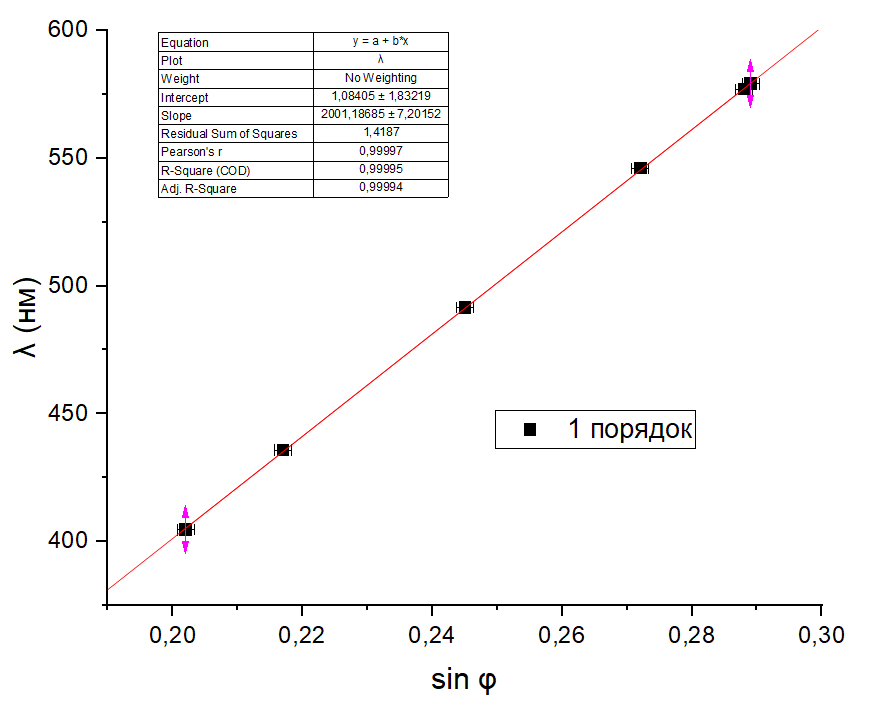
\includegraphics[width=0.5\textwidth]{4.4.1_6.png}&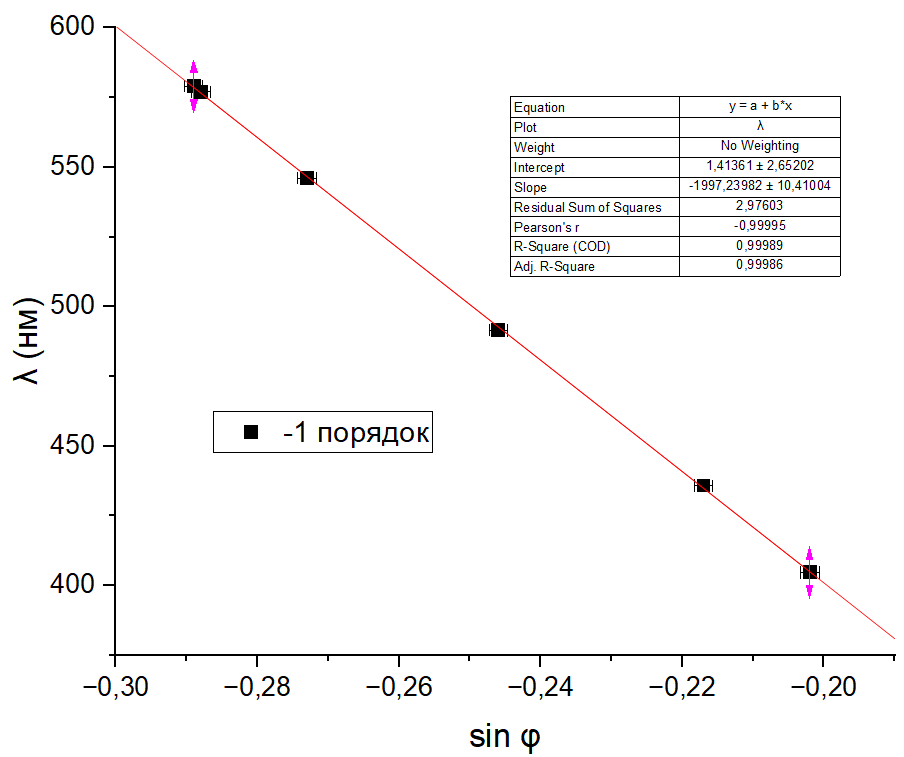
\includegraphics[width=0.5\textwidth]{4.4.1_7.png}\\
\multicolumn{2}{c}{\textbf{Рис. 7.} График зависимости длины волны от угла дифракции для:}\\
а) спектра $1$-го порядка; & б) спектра $2$-го порядка\\
\end{tabular}
\end{center}

\hfill \break Используя формулу (1), для каждого графика, зная коэффициент наклона прямой, определим шаг решетки $d$:

$$
d \sin{\varphi} = m \lambda \rightarrow d = \frac{m\lambda}{\sin{\varphi}} = km,
$$

\hfill \break где $k$ $-$ коэффициент наклона прямой. Коэффициент наклона первого графика ($m = 1$):

$$
k_{1} = (2.001 \pm 0.007) \text{ мкм};
$$

\hfill \break коэффициент наклона второго графика ($m = -1$):

$$
k_{-1} = (-1.997 \pm 0.010) \text{ мкм};
$$

\hfill \break Тогда \textit{шаг решетки}:

$$
d = (1.999 \pm 0.009) \text{ мкм},
$$

\hfill \break что совпадает с приборным значением ($d = 2.00 \text{ мкм}$) в пределах погрешности.

\hfill \break Для оценки \textit{угловой дисперсии} определим угловые координаты линий желтой пары во всех видимых порядках спектра, положительных и отрицательных. Экспериментальную угловую дисперсию рассчитаем по формуле $D = \Delta \varphi / \Delta \lambda$, где $\Delta \lambda \approx 20 \text{\AA} = 20 \cdot 10^{-10} \text{ м}$ $-$ расстояние между центрами желтых линий. 

\begin{center}
\begin{tabular}{|c|c|c|c|c|c|c|}\hline
Порядок & Цвет & $ \varphi $ & $ \Delta \varphi $, угл. сек. & $ D $, угл. сек./$ \text{\AA} $ \\\hline
1 & Желтый (1) & $163^\circ16'22''$ & \multirow{2}{*}{250} & \multirow{2}{*}{12.50} \\\cline{1 -3}
1 & Желтый (2) & $163^\circ12'12''$ & \multirow{2}{*}{} & \multirow{2}{*}{} \\\hline
-1 & Желтый (1) & $196^\circ45'9''$ & \multirow{2}{*}{-226} & \multirow{2}{*}{-11.30} \\\cline{1 -3}
-1 & Желтый (2) & $196^\circ48'55''$ & \multirow{2}{*}{} & \multirow{2}{*}{} \\\hline
2 & Желтый (1) & $144^\circ47'50''$ & \multirow{2}{*}{576} & \multirow{2}{*}{28.80} \\\cline{1 -3}
2 & Желтый (2) & $144^\circ38'14''$ & \multirow{2}{*}{} & \multirow{2}{*}{} \\\hline
-2 & Желтый (1) & $215^\circ14'31''$ & \multirow{2}{*}{-549} & \multirow{2}{*}{-27.45} \\\cline{1 -3}
-2 & Желтый (2) & $215^\circ23'40''$ & \multirow{2}{*}{} & \multirow{2}{*}{} \\\hline
\end{tabular} \\
\hfill \break \textbf {Таблица 2.} Данные для оценки угловой дисперсии\\
\end{center}

\hfill \break Рассчитаем погрешности величин. Во-первых, так как $\Delta \varphi = \varphi_{1} - \varphi_{2}$, то $\sigma_{\Delta \varphi} = \sqrt{\sigma_{\varphi_{1}}^2 + \sigma_{\varphi_{2}}^2}$; во-вторых, $D = \Delta \varphi / \Delta \lambda$, $\Rightarrow$ $\varepsilon_{D} = \varepsilon_{\Delta \varphi}$, то есть $\sigma_{D} = D \cdot \varepsilon_{\Delta \varphi}/100 \% = \frac{D \cdot \sigma_{\Delta \varphi}}{\Delta \varphi}$.

\hfill \break По полученным данным построим график зависимости вида $D = f(m)$, где $m$ $-$ порядок спектра, и проанализируем характер этой зависимости:

\begin{center}
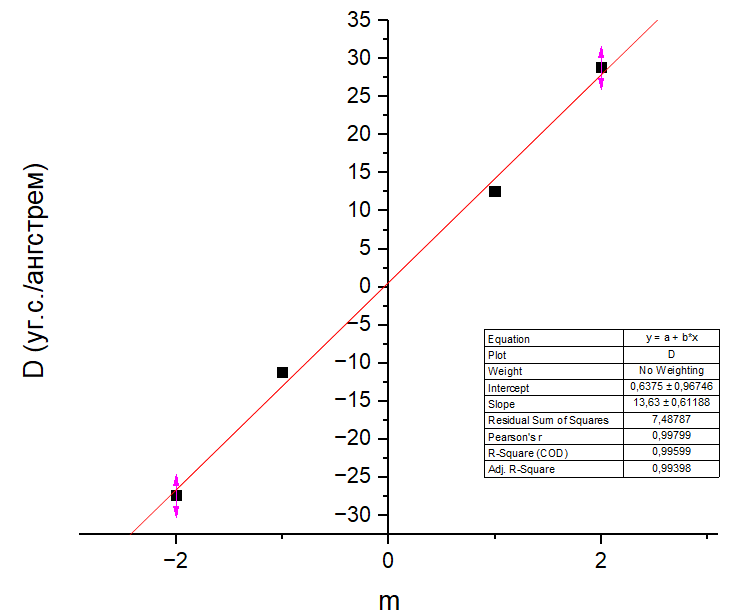
\includegraphics[width=0.65\textwidth]{4.4.1_8.png}\\
\textbf{Рис. 8.} График зависимости вида $D = f(m)$, где $D$ $-$ угловая дисперсия, $m$ $-$ спектральный порядок\\
\end{center}

\hfill \break Видим, что исследуемая зависимость носит линейный характер и график представляется в виде прямой с коэффициентом наклона $k_{\text{эксп}} = (13.63 \pm 0.61$) уг. секунд/\text{\AA} $= (0.66 \pm 0.03)$ 1/мкм. Сравним эту зависимость с рассчитанной по формуле (4) для средней длины волны желтой пары, где для малых углов дифракции дисперсия пропорциональна порядку спектра: $D \approx m/d = m \cdot \frac{1}{d}$, откуда $k_{\text{теор}} = 1/d = (0.50 \pm 0.02)$ 1/мкм, что достаточно близко к экспериментальному значению.

\hfill \break По измерениям координаты и угловой ширины желтой линии определим экспериментальное значение \textit{разрешающей способности} по формуле:

$$
R = \frac{\lambda}{\delta \lambda} = \frac{\varphi}{\delta \varphi} = \frac{D\lambda}{\delta \varphi} = 2890.
$$

\hfill \break Используя формулу (6), оценим число эффективно работающих штрихов $N = R/m = 2890$ и размер освещенной части решетки $l = Nd \approx 5.78 $ мм. Наконец, рассчитаем порядок спектра, при котором фиолетовая линия наложится на желтую. Используя формулу (1) $d\sin{\varphi} = m\lambda$, получим

$$
(m + 1) \lambda_{\text{ф}} = m\lambda_{\text{ж}}
$$

$$
\Rightarrow m = \frac{\lambda_{\text{ф}}}{\lambda_{\text{ж}} - \lambda_{\text{ф}}} \approx 2.34
$$

\section{Вывод}
\hfill \break В ходе эксперимента мы ознакомились с принципами работы гониометра $-$ оптического прибора для точного измерения углов. Был исследован спектр ртутной лампы: в результате измерения угловых координат спектральных линий был экспериментально определен шаг амплитудной решетки $-$ $d = (1.999 \pm 0.009)$ мкм, что неплохо совпадает с фактическим значением $-$ $d = 2.00$ мкм; по угловым координатам линий желтой пары в нескольких спектральных порядках мы сумели оценить угловую дисперсию и убедиться в справедливости формулы $D \approx m/d$ для малых углов дифракции.

\end{document}
